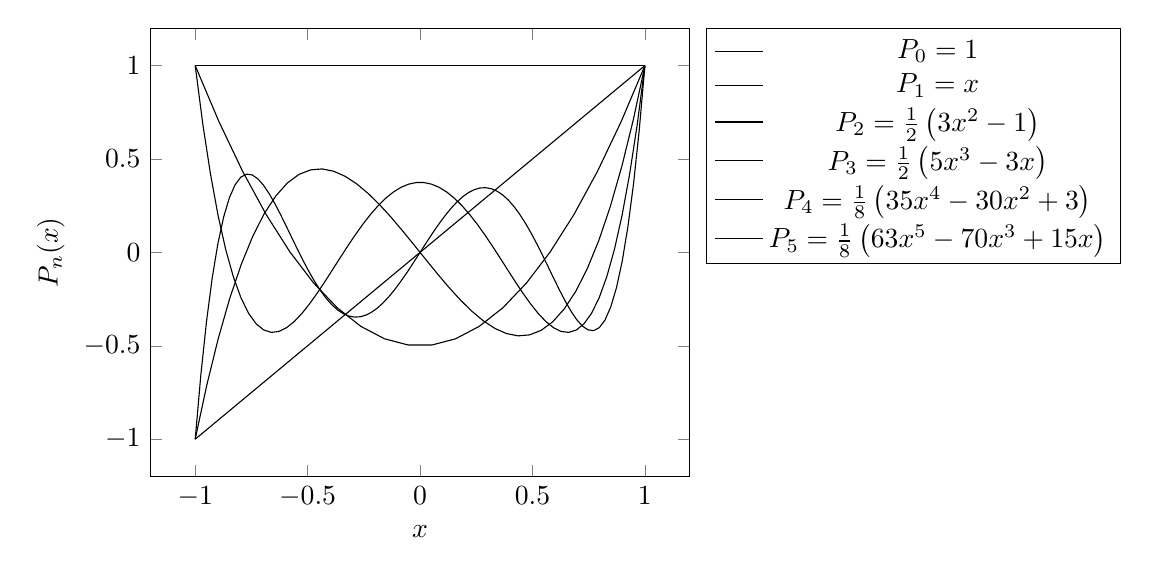
\begin{tikzpicture}
\begin{axis}[
  xlabel=$x$,
  ylabel=$P_n(x)$,
  legend pos = outer north east]
\addplot[samples=2, domain=-1:1] {1};
\addlegendentry{$P_0 = 1$};

\addplot[samples=2, domain=-1:1] {x};
\addlegendentry{$P_1 = x$};

\addplot[samples=20, domain=-1:1] {0.5*(3*x^2-1)};
\addlegendentry{$P_2 = \frac{1}{2} \left( 3x^2 - 1 \right)$};

\addplot[samples=40, domain=-1:1] {0.5*(5*x^3 - 3*x)};
\addlegendentry{$P_3 = \frac{1}{2} \left( 5x^3 - 3x \right)$};

\addplot[samples=60, domain=-1:1] {0.125*(35*x^4 - 30*x^2 + 3)};
\addlegendentry{$P_4 = \frac{1}{8} \left( 35x^4 - 30x^2 + 3 \right)$};

\addplot[samples=80, domain=-1:1] {0.125*(63*x^5 - 70*x^3 + 15*x)};
\addlegendentry{$P_5 = \frac{1}{8} \left( 63x^5 - 70x^3 + 15x \right)$};
\end{axis}
\end{tikzpicture}